\section{Auswertung}

\subsection{Bestimmung von RC anhand einer Entladekurve}

Um RC anhand einer Entladekurve zu bestimmen, wurden am Oszilliskop die Werte in \ref{tab:1} abgelesen. Diese Werte sind auch in graphisch \ref{fig:1} dargestellt.

\begin{figure}[H]
    \centering
    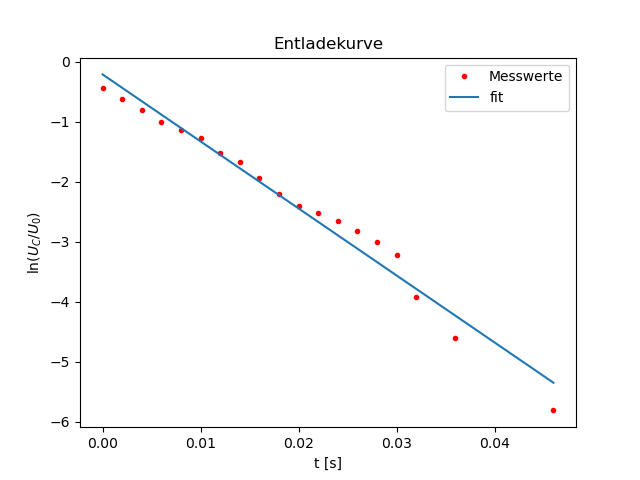
\includegraphics{1.png}
    \label{fig:1}
\end{figure}

\noindent Anschließend wurde eine lineare Ausgleichsrechnung durchgeführt. Dafür wurde eine Formel der folgenden Form verwendet:
\begin{displaymath}
    \ln(\frac{U_C}{U_0}) = -\frac{1}{RC} * t + n 
\end{displaymath}

\noindent Bei dieser Ausgleichsrechnung ergeben sich für folgende Werte für RC und n:
\begin{displaymath}
    RC = 0.00895 \pm 0.00035
\end{displaymath}
\begin{displaymath}
    n = -0.2083 \pm 0.09702
\end{displaymath}

\subsection{Bestimmung von RC mithilfe der Frequenzabhängigkeit der Kondensatorspannung}

Eine weitere Möglichkeit die Zeitkonstante zu bestimmen ist die Frequenzabhängigkeit der Amplitude. Dazu wurde die Ampltude bei verschiedenen Frequenzen abgelesen und wird nun in einem halblogarithmischen Diagramm aufgetragen. Anschließend wird eine nicht lineare Ausgleichsrechnung durchgeführt. Die Formel für diese Ausgleichsrechnung lautet:
\begin{displaymath}
    U_C(\nu) = \frac{a}{\sqrt{1+(RC_2)^2*\nu^2}}
\end{displaymath}

\noindent Dabei ergibt die Ausgleichsrechnung für $RC_2$ = 0.01453$\pm$0.00312.

\subsection{Bestimmung der Zeitkonstante durch die Phasenverschiebung}

Für die dritte und letzte Methode der Bestimmung der Zeitkonstante wird die Phasenverschiebung verwendet. Dabei wurde der Laufzeitunterschied a gemessen. Mit der Formel:
\begin{displaymath}
    \phi = a * \nu * 2*\pi
\end{displaymath}

\noindent wird dieser Laufzeitunterschied in die Phasenverschiebung umgerechnet. Anschließend kann erneut mit einer Ausgleichsrechnung die Zeitkonstnate RC bestimmt werden. Die Ausgleichsrechnung erfolgt mit der Formel:
\begin{displaymath}
    \phi(\nu) = B * \arctan(RC_3*\nu)
\end{displaymath} 

Diese Ausgleichsrechnung liefert $RC_3 = 0.01656 \pm 0.00174$.

Die Werte wurden außerdem nocheinmal graphisch veranschaulicht.

\begin{figure}[H]
    \centering
    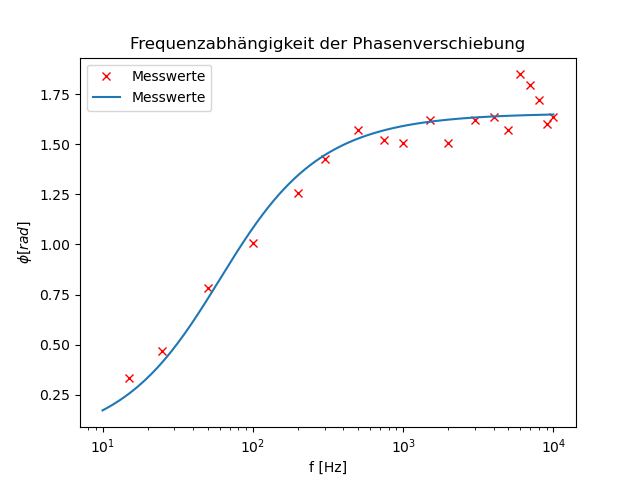
\includegraphics{3.png}
\end{figure}

\section{Diskussion}

Auf drei verschieden Weisen wurde die gleiche Zeitkonstante bestimmt. Dabei sind die folgenden Ergebnisse entstanden.
\begin{align}
    RC_1 = 0.00895 \pm 0.00035 \nonumber \\
    RC_2 = 0.01453 \pm 0.00312 \nonumber \\ 
    RC_3 = 0.01656 \pm 0.00174 \nonumber 
\end{align}

\noindent Dabei ist zu erkennen, dass $RC_2$ und $RC_3$ relativ nah beieinander liegen während $RC_1$ weiter von den anderen entfernt liegt. Konkreter weichen $RC_2$ und $RC_3$ um 12.25\% voneinander ab. $RC_1$ weicht allerdings um 45.95\% von $RC_3$ und um 38,40\% von $RC_2$ ab. 
Dies ist damit zu erklären, dass für den Wert, der über die Entladekurve bestimmt worden ist, alle Werte vom Oszilloskop abgelesen werden mussten. Bei der Frequenzabhängigkeit und der Phasenverschiebung wurde immerhin mit der Frequenz gearbeitet. Diese lies sich sehr genau einstellen, sodass der Ablesefehler, welcher durch das Ablesen der Werte am Oszilloskop entsteht, in einem Wert weniger auftaucht. Der Am Oszilloskop entstehende Ablesefehler ist dabei sehr groß. Dies liegt daran, dass am Oszilloskop keine feine Auflösung einstellbar ist. Außerdem ist die zu sehende Linie relativ breit. Dieser Umstande erschwert das Ablesen zusätzlich. 
Unter Betrachtung dieser Ableseungenauigkeit sind $RC_2$ und $RC_3$ gut bestimmt. Der Wert für $RC_1$ allerdings lässt nur die Vermutung auf einen systematischen Fehler zu. Es muss bei der Messung ein Fehler wie eine falsche Eichung des Oszilloskops entstanden sein, denn reine Ableseungenauigkeiten und andere gewöhnliche Messungenauigkeiten erklären eine so große Abweichung nicht. 


\section{Tabellen}

\begin{minipage}{\linewidth}
    \begin{table}[H]
        \centering
    \captionof{table}{Wertepaare aus der Entladekurve}
    \begin{tabular}{ll}
        \toprule
        Zeit [ms] & Spannung [V]  \\
        \midrule
        0      & 0.65 \\
        2      & 0.54 \\
        4      & 0.45 \\
        6      & 0.37 \\
        8      & 0.32 \\
        10     & 0.28 \\
        12     & 0.22 \\
        14     & 0.19 \\
        16     & 0.145\\
        18     & 0.11 \\
        20     & 0.09 \\
        22     & 0.08 \\
        24     & 0.07 \\
        26     & 0.06 \\
        28     & 0.05 \\
        30     & 0.04 \\
        32     & 0.02 \\
        36     & 0.01 \\
        46     & 0.003\\
        \bottomrule   
    \end{tabular}
    
    \label{tab:1}
\end{table}
\end{minipage}
